83. $(x^2-4x-5)\left(\cfrac{x}{x^2-5x+6}+\cfrac{5}{x^2-10x+21}+\cfrac{7}{(x-2)(x-3)(x-7)}
ight)\geqslant0\Leftrightarrow$\\$
(x-5)(x+1)\left(\cfrac{x}{(x-2)(x-3)}+\cfrac{5}{(x-3)(x-7)}+\cfrac{7}{(x-2)(x-3)(x-7)}
ight)\geqslant0\Leftrightarrow$\\$
(x-5)(x+1)\cdot\cfrac{x^2-7x+5x-10+7}{(x-2)(x-3)(x-7)}\geqslant0\Leftrightarrow
\cfrac{(x-5)(x+1)(x^2-2x-3)}{(x-2)(x-3)(x-7)}\geqslant0\Leftrightarrow
\cfrac{(x-5)(x+1)^2(x-3)}{(x-2)(x-3)(x-7)}\geqslant0.$ Применив метод интервалов, найдём ответ: $x\in\{-1\}\cup(2;3)\cup(3;5]\cup(7;+\infty).$
\begin{figure}[ht!]
\center{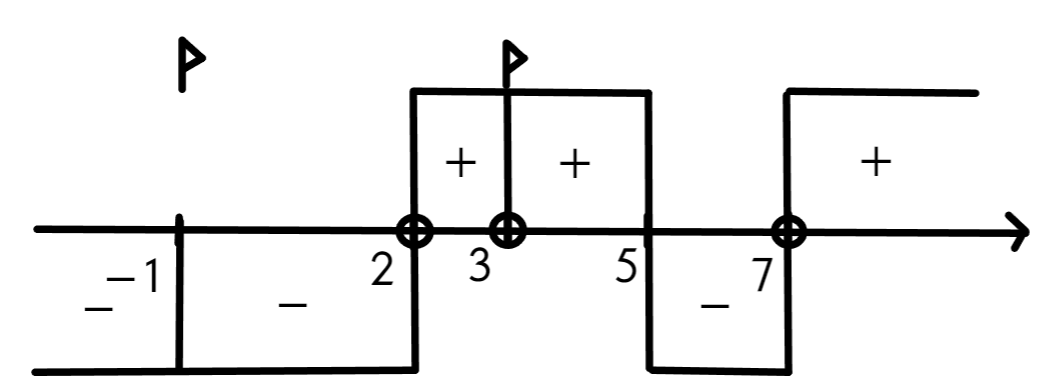
\includegraphics[scale=0.35]{ner9-833.png}}
\end{figure}\\
